\subsection{The Decremental Algorithm}
\label{dec}

The decremental algorithm, denoted by {\tt Dec}, differs from previous query algorithms
not only on the generation of candidate keyword sets,
but also on the verification of candidate keyword sets.

\textbf{1. Generation of candidate keyword sets.}
{\tt Dec} exploits the key observation that,
if $S'$ ($S'\subseteq S$) is a qualified keyword set,
then there are at least $k$ of $q$'s neighbors containing set $S'$.
This is because every vertex in $G_k[S']$ must has degree at least $k$.
This observation implies,
we can generate all the candidate keyword sets directly by using the query vertex $q$ and $q$'s neighbors,
without touching other vertices.

Specifically, we consider $q$ and $q$'s neighbor vertices.
For each vertex $v$, we only select the keywords, which are contained by $S$ and at least $k$ of its neighbors.
Then we use these selected keywords to form an itemset, in which each item is a keyword.
After this step, we obtain a list of itemsets.
Then we apply the well studied frequent pattern mining algorithms
(e.g., Apriori~\cite{han2011data} and FP-Growth~\cite{han2000mining})
to find the frequent keyword combinations,
each of which is a candidate keyword set.
Since our goal is to generate keyword combinations shared by at least $k$ neighbors,
we set the minimum support as $k$.
In this paper, we use the well-known FP-Growth algorithm~\cite{han2000mining}.

\begin{figure}[ht]
    \centering
    \mbox{
        \subfigure[a query vertex]{
            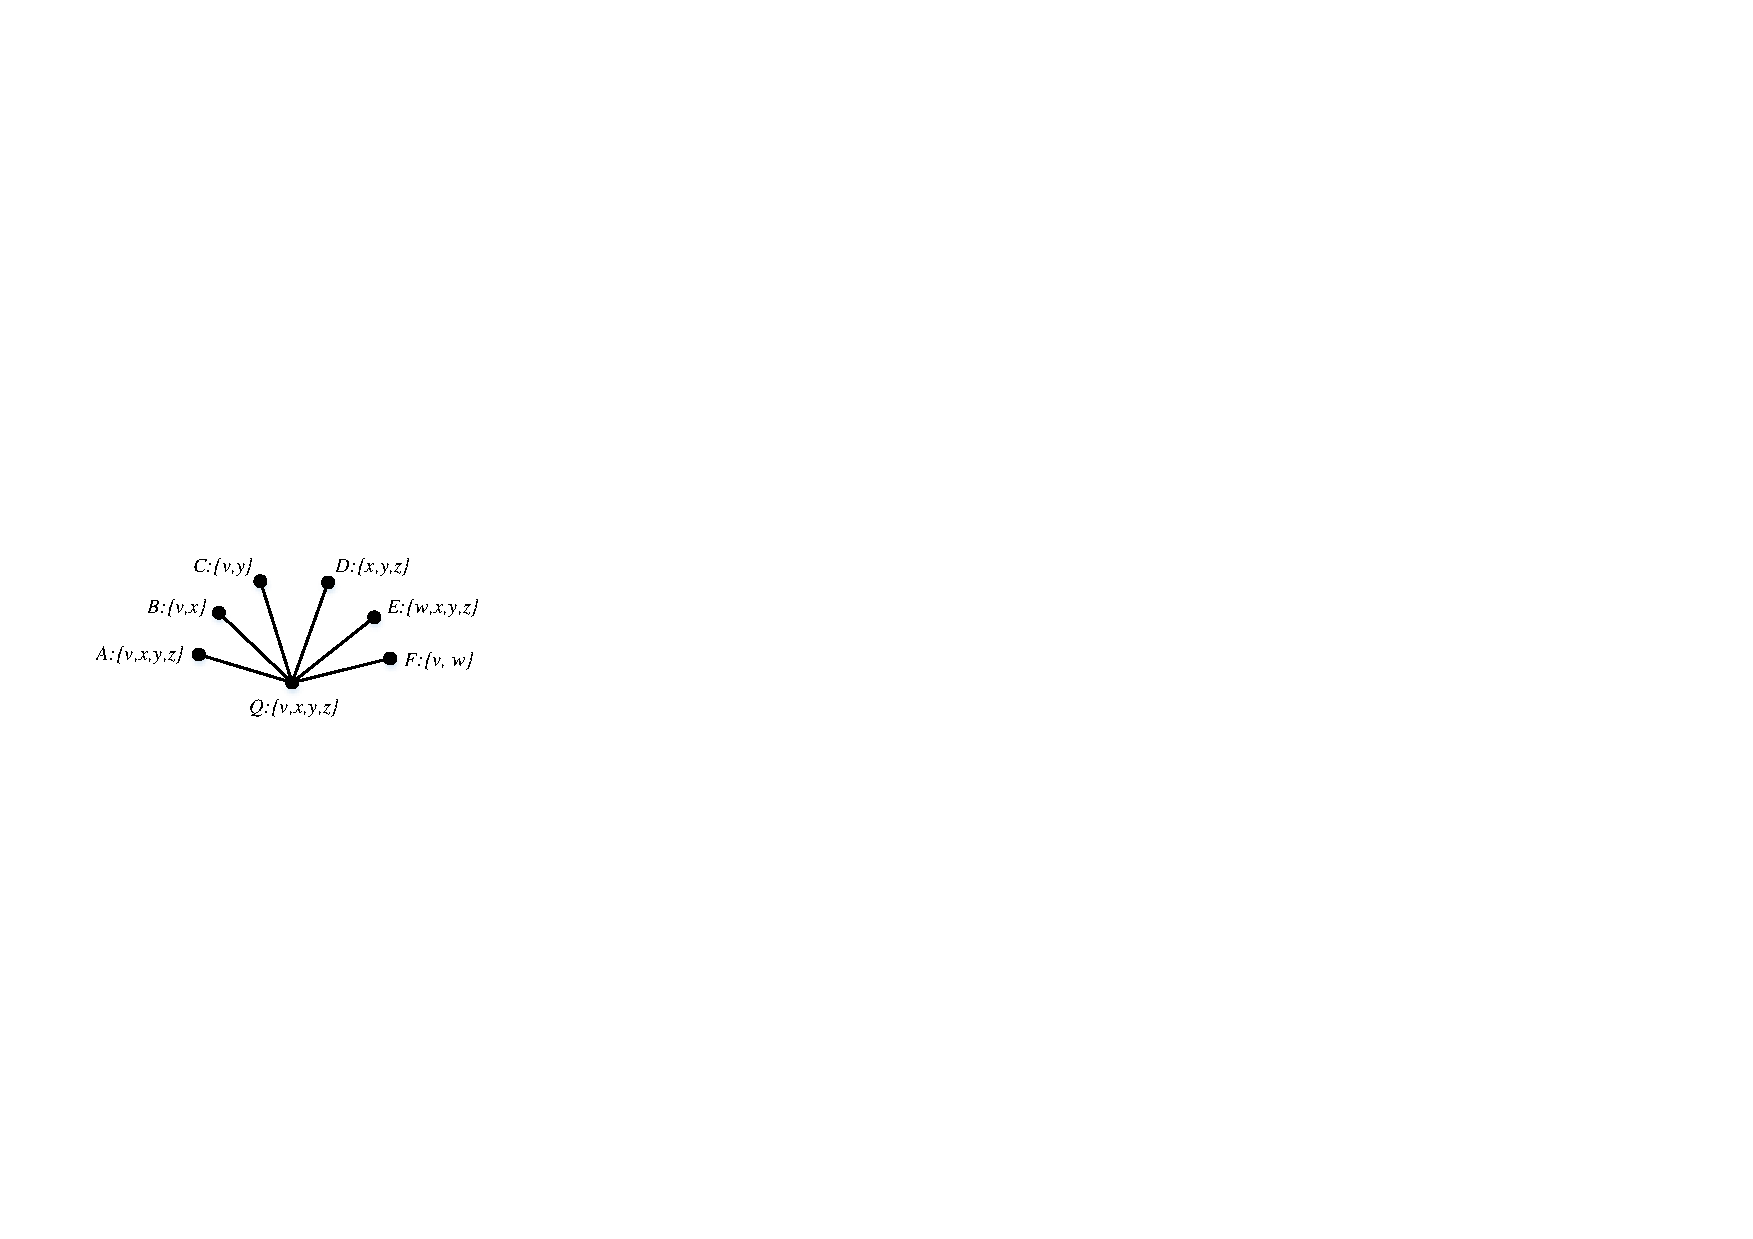
\includegraphics[width=.51\columnwidth]{figures/nghGraph}
            \label{fig:nghGraph}
        }
        \hspace{1ex}
        \subfigure[candidates]{
            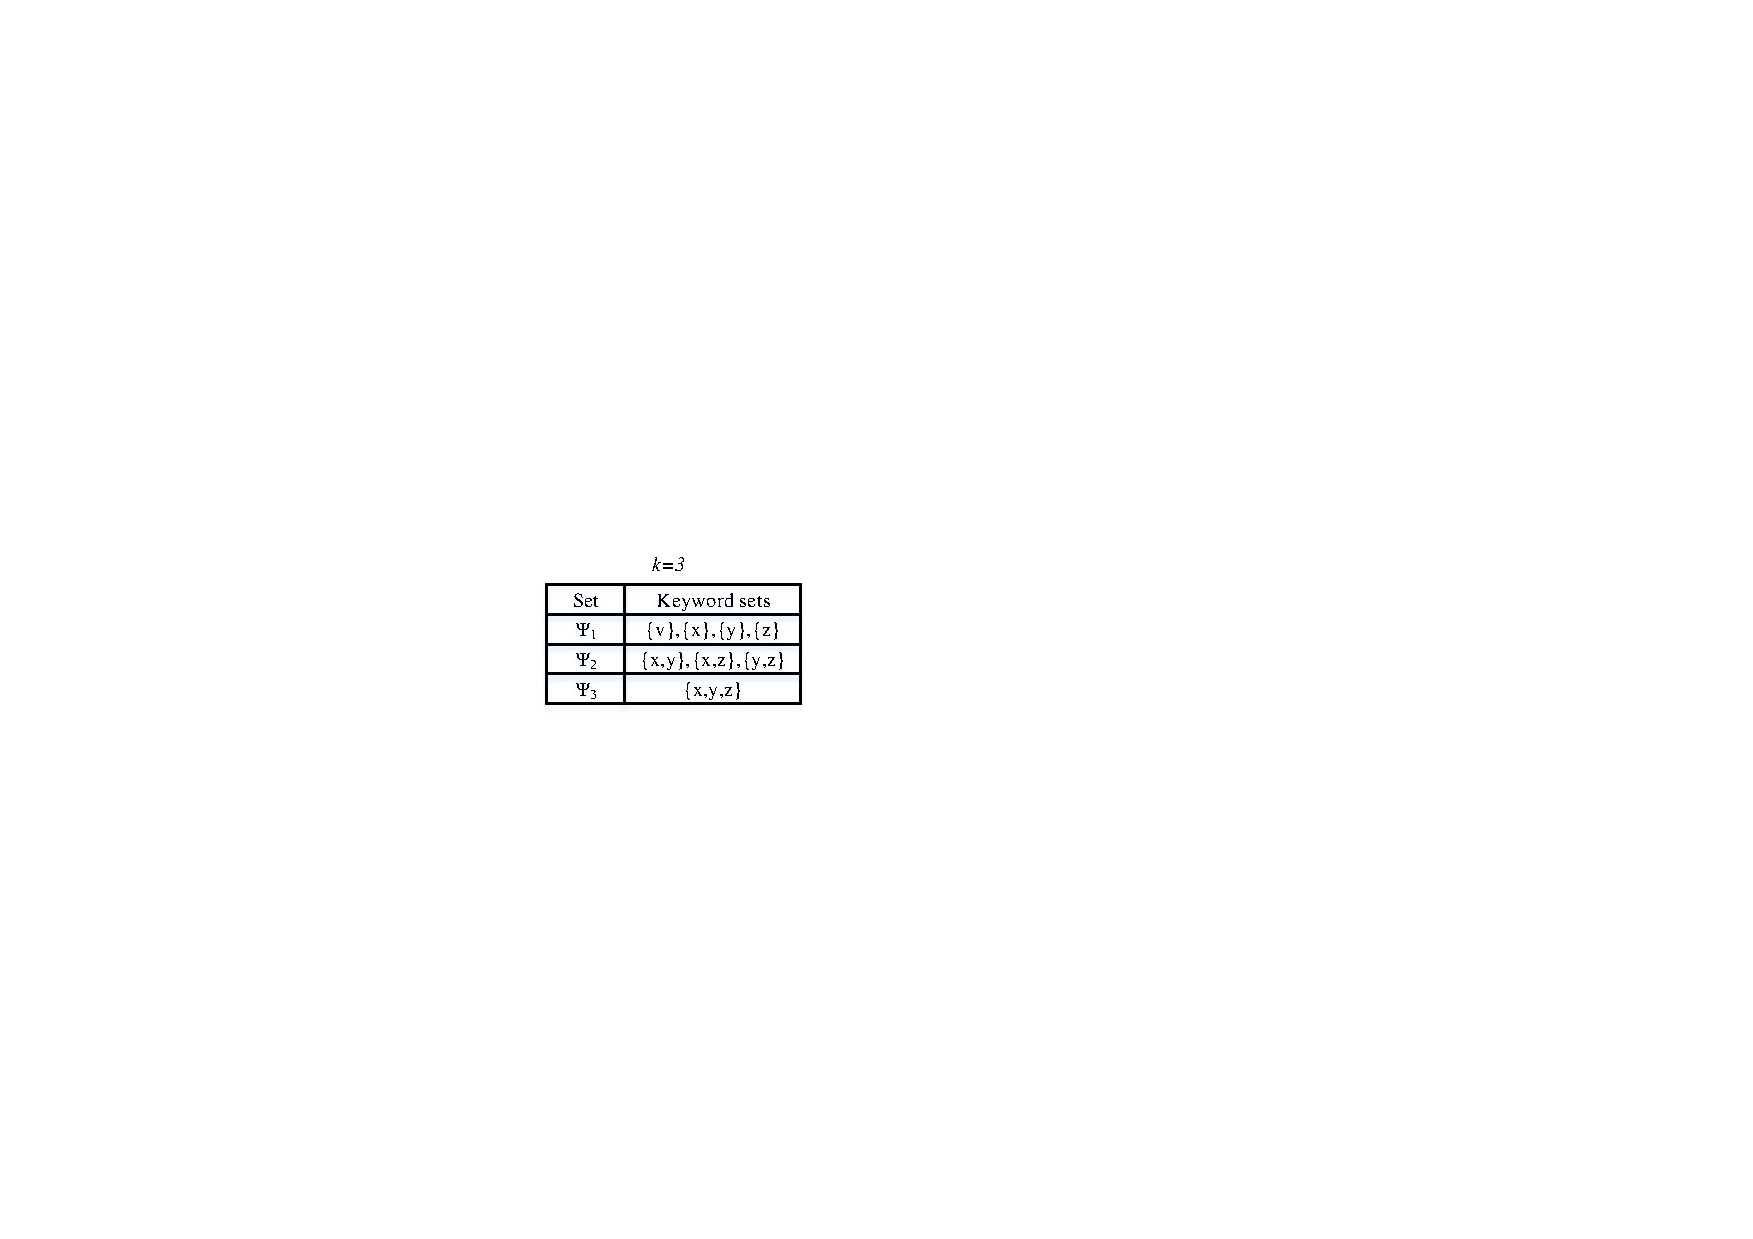
\includegraphics[width=.34\columnwidth]{figures/nghCand}
            \label{fig:nghCand}
        }
    }
    \caption{An example of candidate generation.}
\end{figure}
\begin{example}
Consider a query vertex $Q$ ($k$=3, $S$=$\{v,x,y,z\}$) with 6 neighbors in Figure~\ref{fig:nghGraph},
where the selected keywords of each vertex are listed in curly braces.
By FP-Growth, 8 candidate keyword sets are generated, as shown in Figure~\ref{fig:nghCand}.
$\Psi_i$ denotes the set of keyword sets with sizes being $i$.
\end{example}

\textbf{2. Verification of candidate keyword sets.}
As candidates can be obtained using $S$ and $q$'s neighbors directly,
we can verify them either incrementally as that in {\tt Inc-S},
or in a decremental manner (larger candidate keyword sets first and smaller candidate keyword sets later).
In this paper, we choose the latter manner. The rationale behind is that,
for any two keyword sets $S_1\subseteq S_2$, the number of vertices containing $S_2$ is usually smaller than that of $S_1$,
which implies $S_2$ can be verified more efficiently than $S_1$.

\begin{algorithm}[h]
\caption{Query algorithm: {\tt Dec}}
\label{alg:ngh}
\footnotesize{
\algrenewcommand{\algorithmiccomment}[1]{\hskip3em$//$ #1}
\begin{algorithmic}[1]
    \Function{query($G$, $root$, $q$, $k$, $S$)}{}
        \State generate $\Psi_1,\Psi_2,\cdots, \Psi_h$ using $S$ and $q$'s neighbors;
        \State find the subtree root node $r_k$;
        \State create $R_1,R_2,\cdots,R_{h'}$ by using subtree rooted at $r_k$;
        \State $l\gets h$; $Q\gets \emptyset$;
        \State ${\widehat R}\gets {R_h} \cup \cdots \cup {R_{h'}}$;
        \While {$l\geq 1$}
            \For {each $S'\in \Psi_l$}
                \State find $G[S']$ from the subgraph induced on $\widehat R$;
                \State find $G_k[S']$ from $G[S']$;
                \If {$G_k[S']$ exists}
                    $Q$.add($G_k[S']$);
                \EndIf
            \EndFor
            \If {$Q$=$\emptyset$}
                \State $l\gets l-1$;
                \State ${\widehat R}\gets {\widehat R}\cup R_l$;
            \Else {} break;
            \EndIf
        \EndWhile
        \State output communities in $Q$;
    \EndFunction
\end{algorithmic}}
\end{algorithm}

Based on the above discussions, we design {\tt Dec} as shown in Algorithm~\ref{alg:ngh}.
We first generate candidate keyword sets using $S$ and $q$'s neighbors by FP-Growth algorithm (line 2).
Then, we apply {\tt core-locating} to find the root (with core number $k$) of the subtree from CL-tree,
whose corresponding $k$-$\widehat {core}$ contains $q$ (line 3).
Next, we traverse the subtree rooted at $r_k$
and find vertices which share keywords with $q$ (line 4).
$R_i$ denote the sets of vertices sharing $i$ keywords with $q$.
Then, we initialize $l$ as $h$ (line 5),
as we verify keyword sets with the largest size $h$ first.
We maintain a set $\widehat R$ dynamically,
which contains vertices sharing at least $l$ keywords with $q$ (line 6).
In the while loop, we examine candidate keyword sets in the decremental manner.
For each candidate $S'\in\Psi_l$, we first try to find $G[S']$, then find $G_k[S']$,
and put $G_k[S']$ into $Q$ if it exists (lines 8-11).
Finally, if we have found at least one qualified community,
we stop at the end of this loop and output $Q$;
otherwise, we examine smaller candidate keyword sets in next loop. 